
\subsection{Photon identification with Neural Network}
\begin{frame}{EM calorimeter and $\gamma$ object}
\begin{columns}
\column{0.4\textwidth}
\begin{figure}
    \centering
    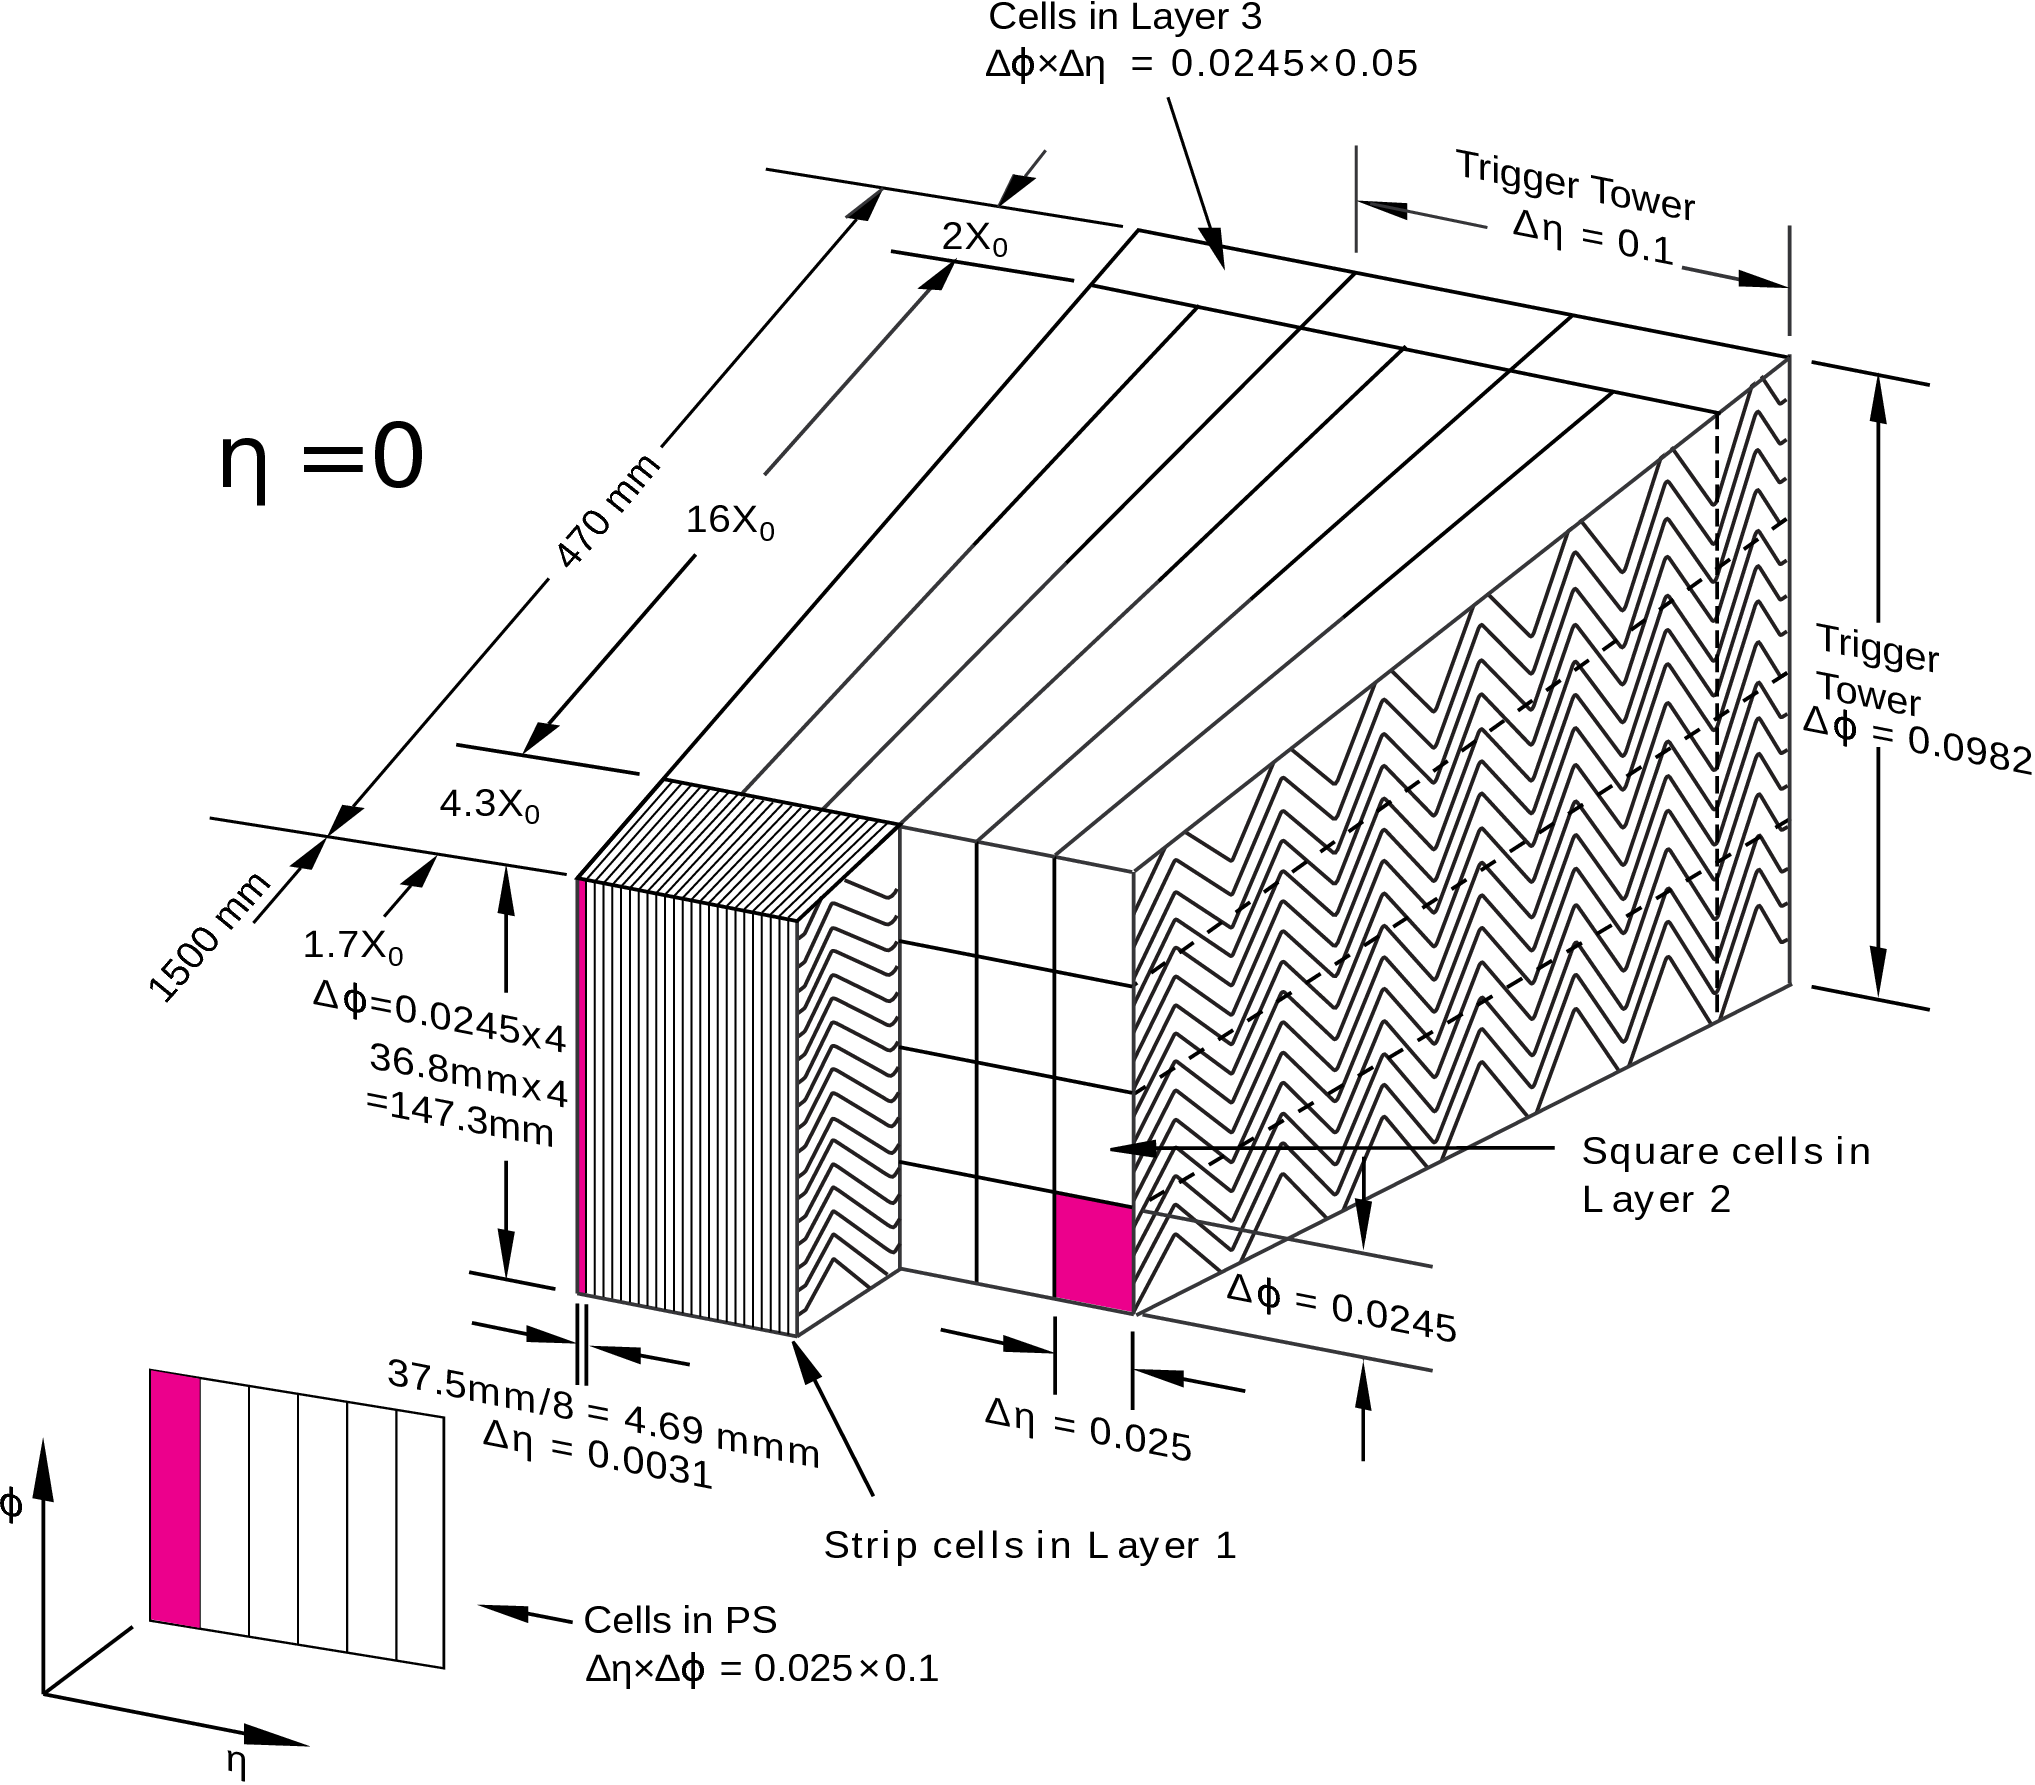
\includegraphics[width=1.\textwidth]{Part6/Img/EM.png}
\end{figure}
\column{0.6\textwidth}

\begin{itemize}
    \item \textcolor{structurColor}{\textbf{3 layers}} with different \textbf{cell size} (+ Presampler)
    \item \textbf{$N_{\eta}\times N_{\phi}$ cluster} (around the hottest cell) contains $\gamma$ energy
    \pause
    \item \textcolor{HHturquoise_d}{\textbf{Shower shapes}} (SS) quantities ($\sim$ 11) evaluated from 7$\times$11 cluster
    \begin{itemize}
        \item \textbf{lateral} \& \textbf{longitudinal} EM shower
        \item \textbf{encode separation}: \textcolor{HHred}{\textbf{prompts}} vs \textcolor{HHblue}{\textbf{background}} (QCD jets)
    \end{itemize}
\end{itemize}
\visible<2-3>{
\begin{figure}
    \centering
    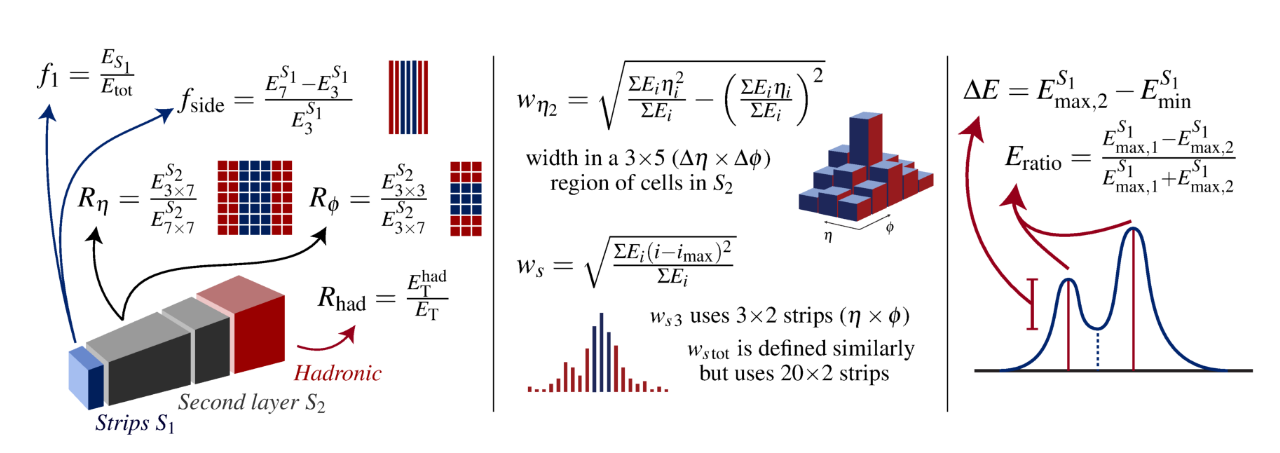
\includegraphics[width=0.8\textwidth]{Part6/Img/ShowerShapes.png}
\end{figure}
}
\pause
\begin{itemize}
    \item Identification relies on SS: \textbf{cut-based algorithm}
    \item \textcolor{HHred}{\textbf{Improvement using Neural Network}}
\end{itemize}
\end{columns} 
\end{frame}

\begin{frame}{Photon identification with Neural Network}
\begin{columns}
\column{0.6\textwidth}    
\begin{itemize}
    \item \textbf{cut-based $\to$ DNN} (High level)
    \begin{itemize}
        \item \textcolor{HHred}{\textbf{limited performance}} (small features space)
    \end{itemize}
    \pause
    \item solution: \textbf{\textcolor{HHturquoise_d}{breakdown to cell level}} (Low level)
    \begin{itemize}
        \item scale up features space dimensionality
        \begin{itemize}
            \item \textbf{generate more variables}
            \item \textbf{correlation}
        \end{itemize} 
    \end{itemize}
    \pause
    \item \textcolor{structurColor}{\textbf{Convolutional Neural Network (CNN)}}
    \begin{itemize}
        \item photon cluster represented as an image
    \end{itemize}
    \item Photon identification using images from the 3 layers 
\end{itemize}    
\column{0.4\textwidth}  

\visible<3>{
\begin{figure}
        \centering
        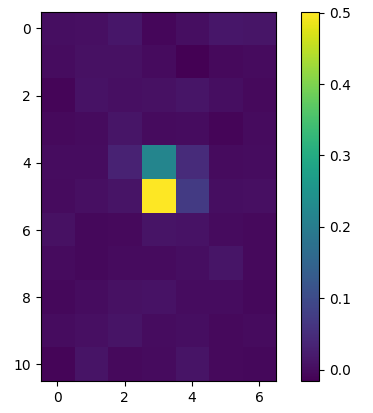
\includegraphics[width=0.8\textwidth]{Part6/Img/7_11_cluster.png}
\end{figure}
}

\end{columns}
\end{frame}

\begin{frame}{Convolutional Neural Network strategy and training}
\begin{columns}
\column{0.6\textwidth}    
\begin{itemize}
    \item \textcolor{HHred}{\textbf{prompts photons}}: inclusive $\gamma$+jets events
    \item \textcolor{HHblue}{\textbf{background photons}}: QCD di-jet events 
    \item + truth matching 
    \pause
    \item images from \textbf{7$\times$11 windows} 
    \begin{itemize}
        \item \textbf{energy independent algorithm}
        \item image pixel = cell energy fraction
    \end{itemize}
    \pause
    \item \textbf{inclusive training} ($E_T$, $\eta$, conversion type)
    \item \textbf{2 NVIDIA Tesla K80 GPUs}
    \end{itemize}
    \pause
    \begin{itemize}
        \item CNN \textcolor{HHred}{\textbf{over-performs}} the cut-based algorithm
        \item \textbf{An improvement of up to 93\%}
    \end{itemize}
    
    
\column{0.4\textwidth} 

\begin{figure}
    \begin{overprint}
    \onslide<1-3>\centering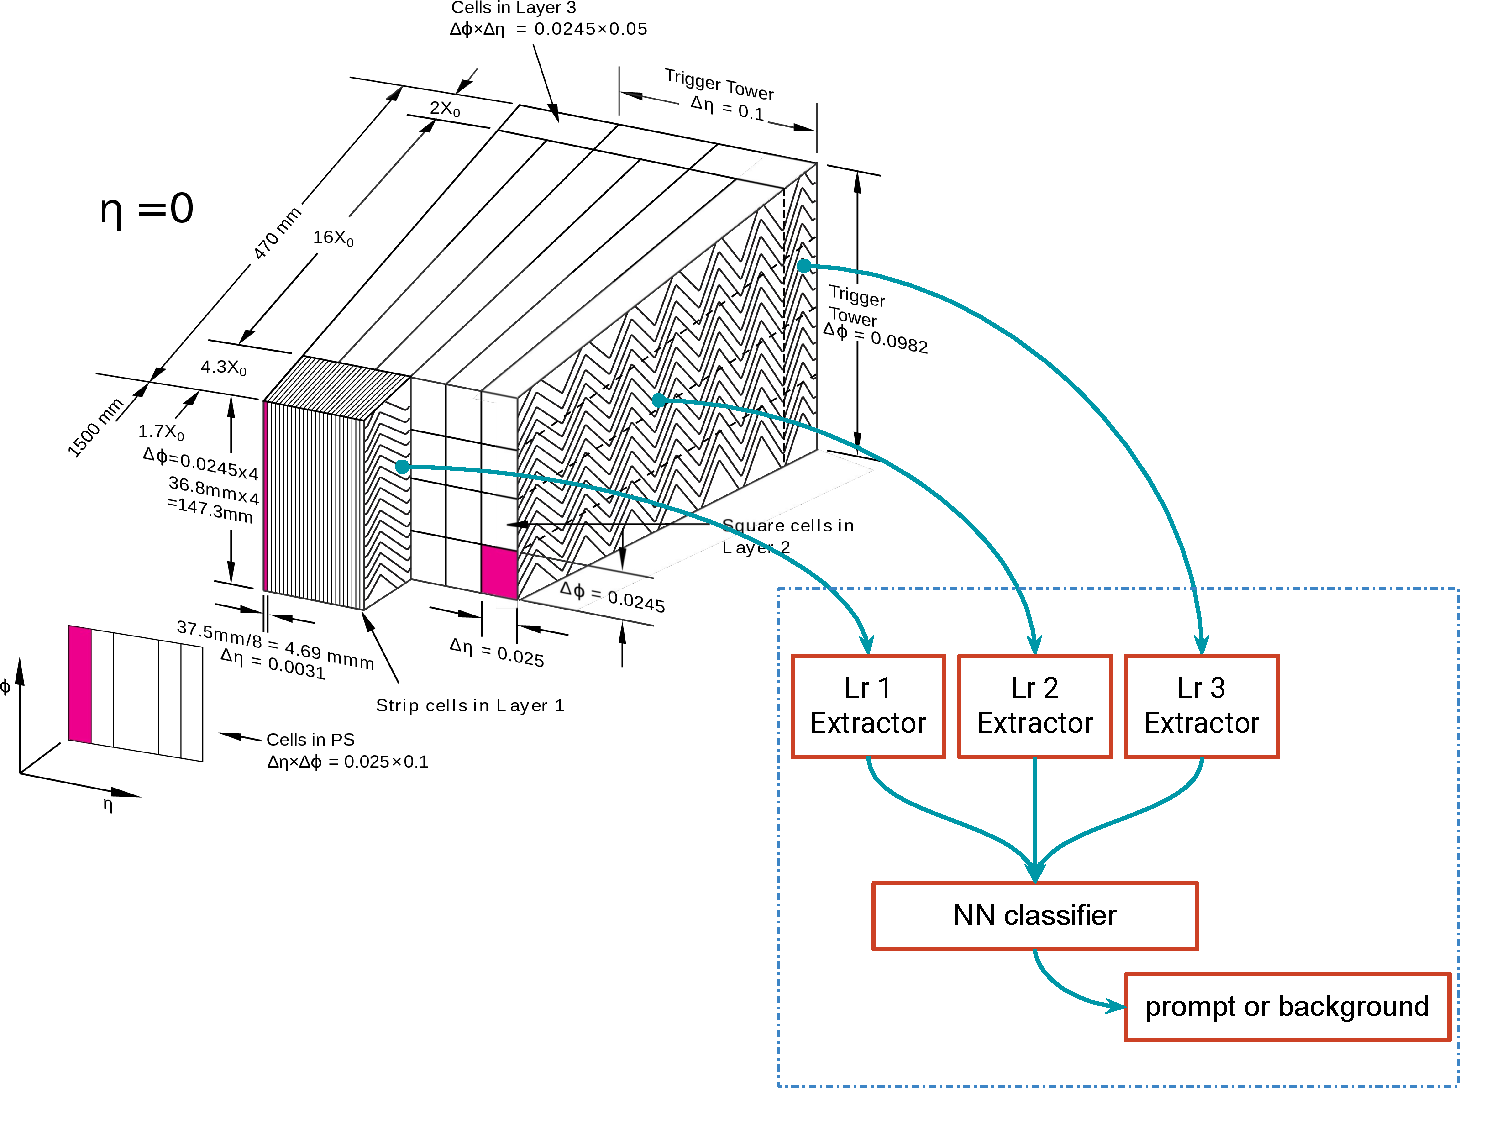
\includegraphics[width=1.1\textwidth]{Part6/Img/CNN_Idea2.pdf}
    \onslide<4>\centering\fcolorbox{HHred}{HHwhite2}{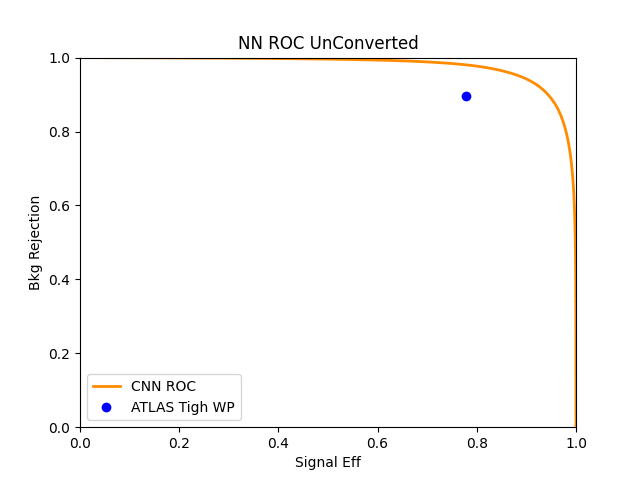
\includegraphics[width=1\textwidth]{Part6/Img/ROC_UnConverted.png}}
    \end{overprint}
\end{figure}
\end{columns}
\end{frame}

\subsection{identification efficiency and scale factors}
\begin{frame}{Photon identification efficiency}
\begin{columns}
\column{0.6\textwidth}

\begin{itemize}
    \item identification efficiency with \textcolor{HHred}{\textbf{Radiative Z method}} 
    \begin{itemize}
        \item Z$\to ll\gamma$, \textbf{as a signal}
        \item Z$\to ll$+jet, \textbf{as a background}
        \item \textbf{2017 data} (43.6 fb$^{-1}$)
    \end{itemize}
    \item efficiency as
    \begin{equation*}
        \epsilon_{ID} = \frac{N^{\text{after ID}} \times P^{\text{after ID}}}{N^{\text{before ID}} \times P^{\text{before ID}}}
    \end{equation*}
    
    \item purity estimated with \textcolor{HHturquoise_d}{\textbf{template fit of $m_{ll\gamma}$}}
    \begin{itemize}
        \item signal template \textbf{from Monte Carlo}
        \item \textbf{second-order polynomial function} for background
        \item \textcolor{structurColor}{\textbf{$E_T^{\gamma} > $ 30 GeV, pure photon samples}} 
    \end{itemize}
    \onslide<4>{
    \item \textcolor{HHred}{\textbf{over-performs}} the cut-based algorithm
    \begin{itemize}
        \item out-of-sample validation: \textbf{different event topology}
        \item \textbf{good data-MC agreement}, scale factor close to unity
    \end{itemize}
    }
\end{itemize}

\column{0.4\textwidth}

\begin{figure}
    \begin{overprint}
    \onslide<2>\centering\fcolorbox{HHturquoise_d}{HHwhite2}{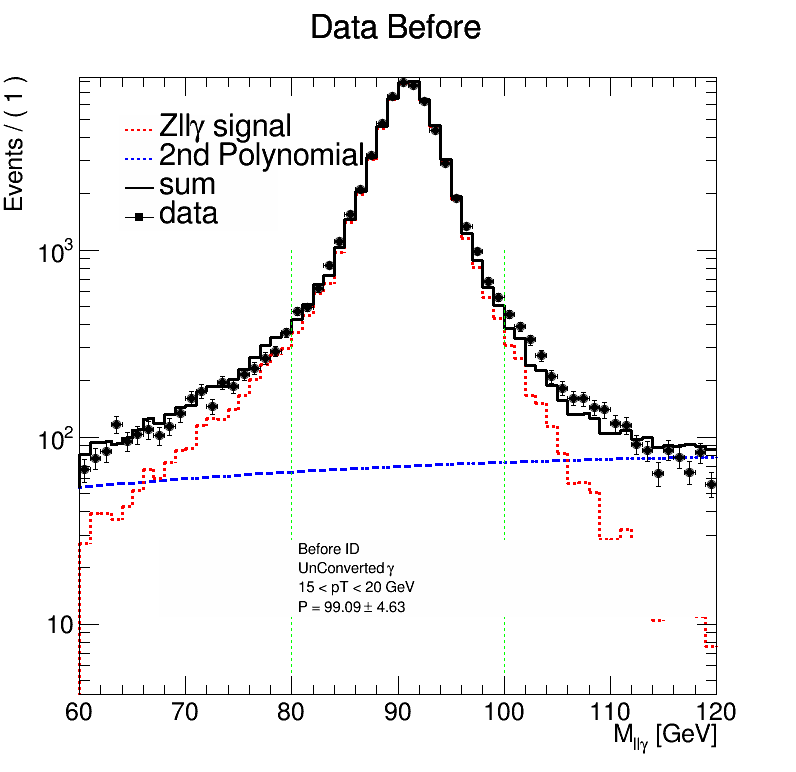
\includegraphics[width=1.\textwidth]{Part6/Img/UnConvertedllg_Before_ID_Bin_1.png}}
    \onslide<3>\centering\fcolorbox{structurColor}{HHwhite2}{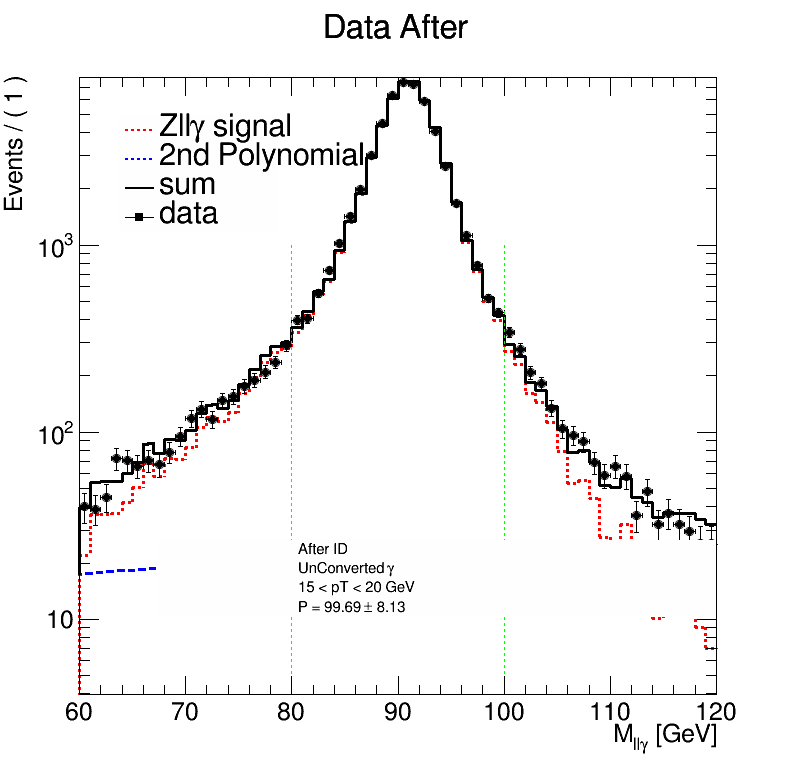
\includegraphics[width=1.\textwidth]{Part6/Img/UnConvertedllg_After_ID_Bin_1.png}}
    \onslide<4->\centering\fcolorbox{HHred}{HHwhite2}{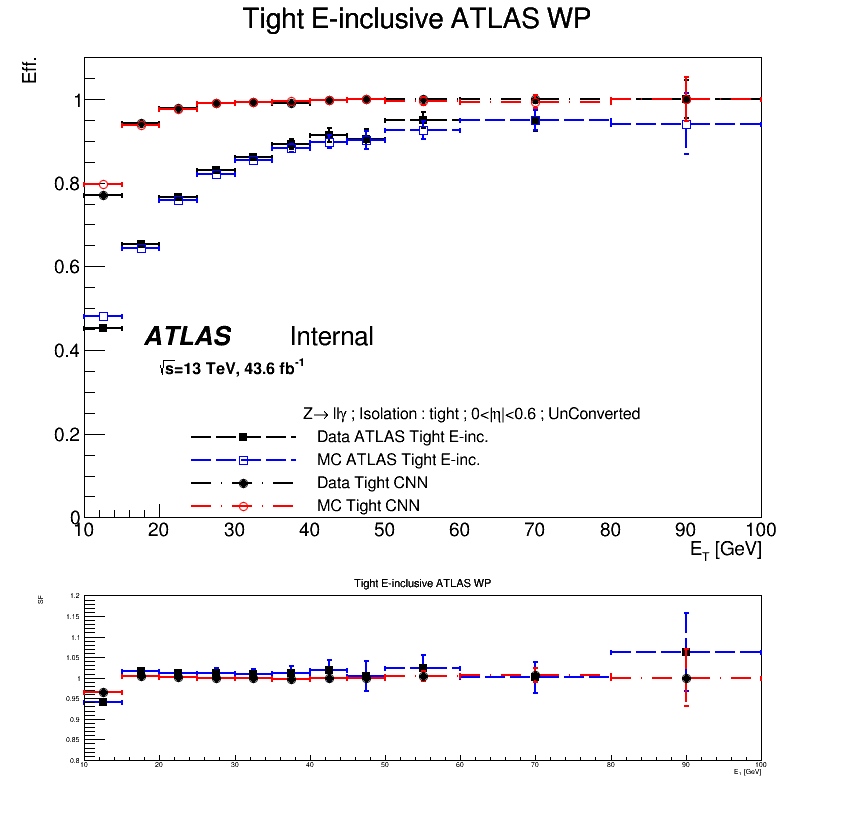
\includegraphics[width=1.\textwidth]{Part6/Img/Tight_Inc_vs_Tight_CNN__UnConverted_Iso_tight_Wgt_ETA_Bin_1.png}}
    \end{overprint}
\end{figure}

\end{columns}
\end{frame}

%\subsection{Impact on HH$\to b\bar{b}\gamma\gamma$}
\begin{frame}{Impact on HH$\to b\bar{b}\gamma\gamma$ analysis}
\begin{columns}
\column{0.6\textwidth}    
\begin{itemize}
    \item CNN applied to photons from HH$\to b\bar{b}\gamma\gamma$ signal
    \begin{itemize}
    \onslide<2->{
        \item \textcolor{HHturquoise_d}{\textbf{efficiency close to 100\%}}
    }
    \onslide<3->{
        \item \textbf{15\% improvement in signal acceptance}
    }    
    \end{itemize}
    \onslide<4->{
    \item CNN applied to photons from continuum $\gamma\gamma$+jets
    }
    \begin{itemize}
    \onslide<5->{
        \item \textcolor{HHturquoise_m}{\textbf{high $\gamma\gamma$ purity}}
    }
   \onslide<6->{    
        \item \textbf{15\% increase in statistics}
    }    
    \end{itemize}
    \onslide<7->{
    \item \textbf{\textcolor{HHred}{$\sim$ 7.3\%} improvement in analysis significance}
    \item \textbf{reduce background modelling systematics}
    }
\end{itemize}
\column{0.4\textwidth}    

\begin{figure}
    \begin{overprint}
    \onslide<2>\centering\fcolorbox{HHturquoise_d}{HHwhite2}{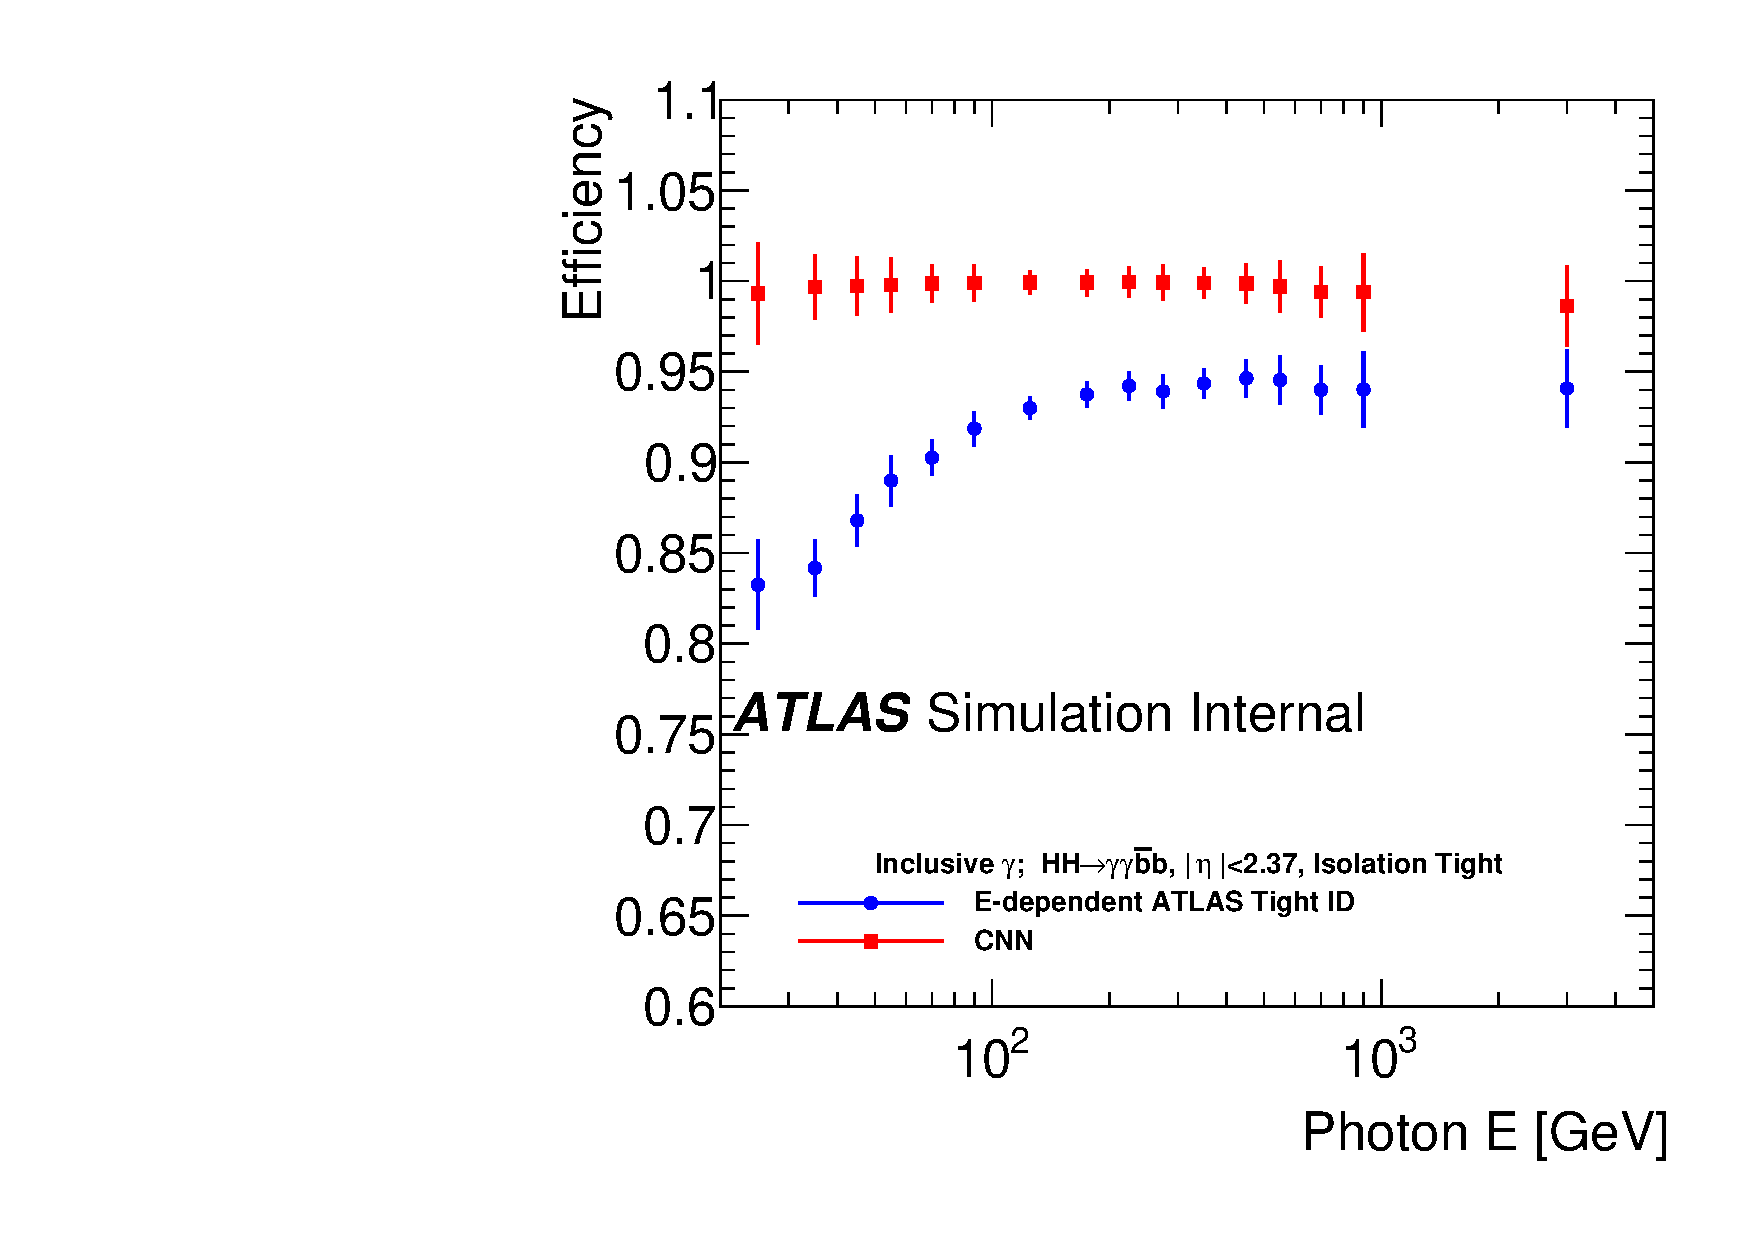
\includegraphics[width=1\textwidth]{Part6/Img/Eff_Tight_All_Inclusive_Tight_E_Sig.pdf}}
    \onslide<3>\centering\fcolorbox{HHturquoise_d}{HHwhite2}{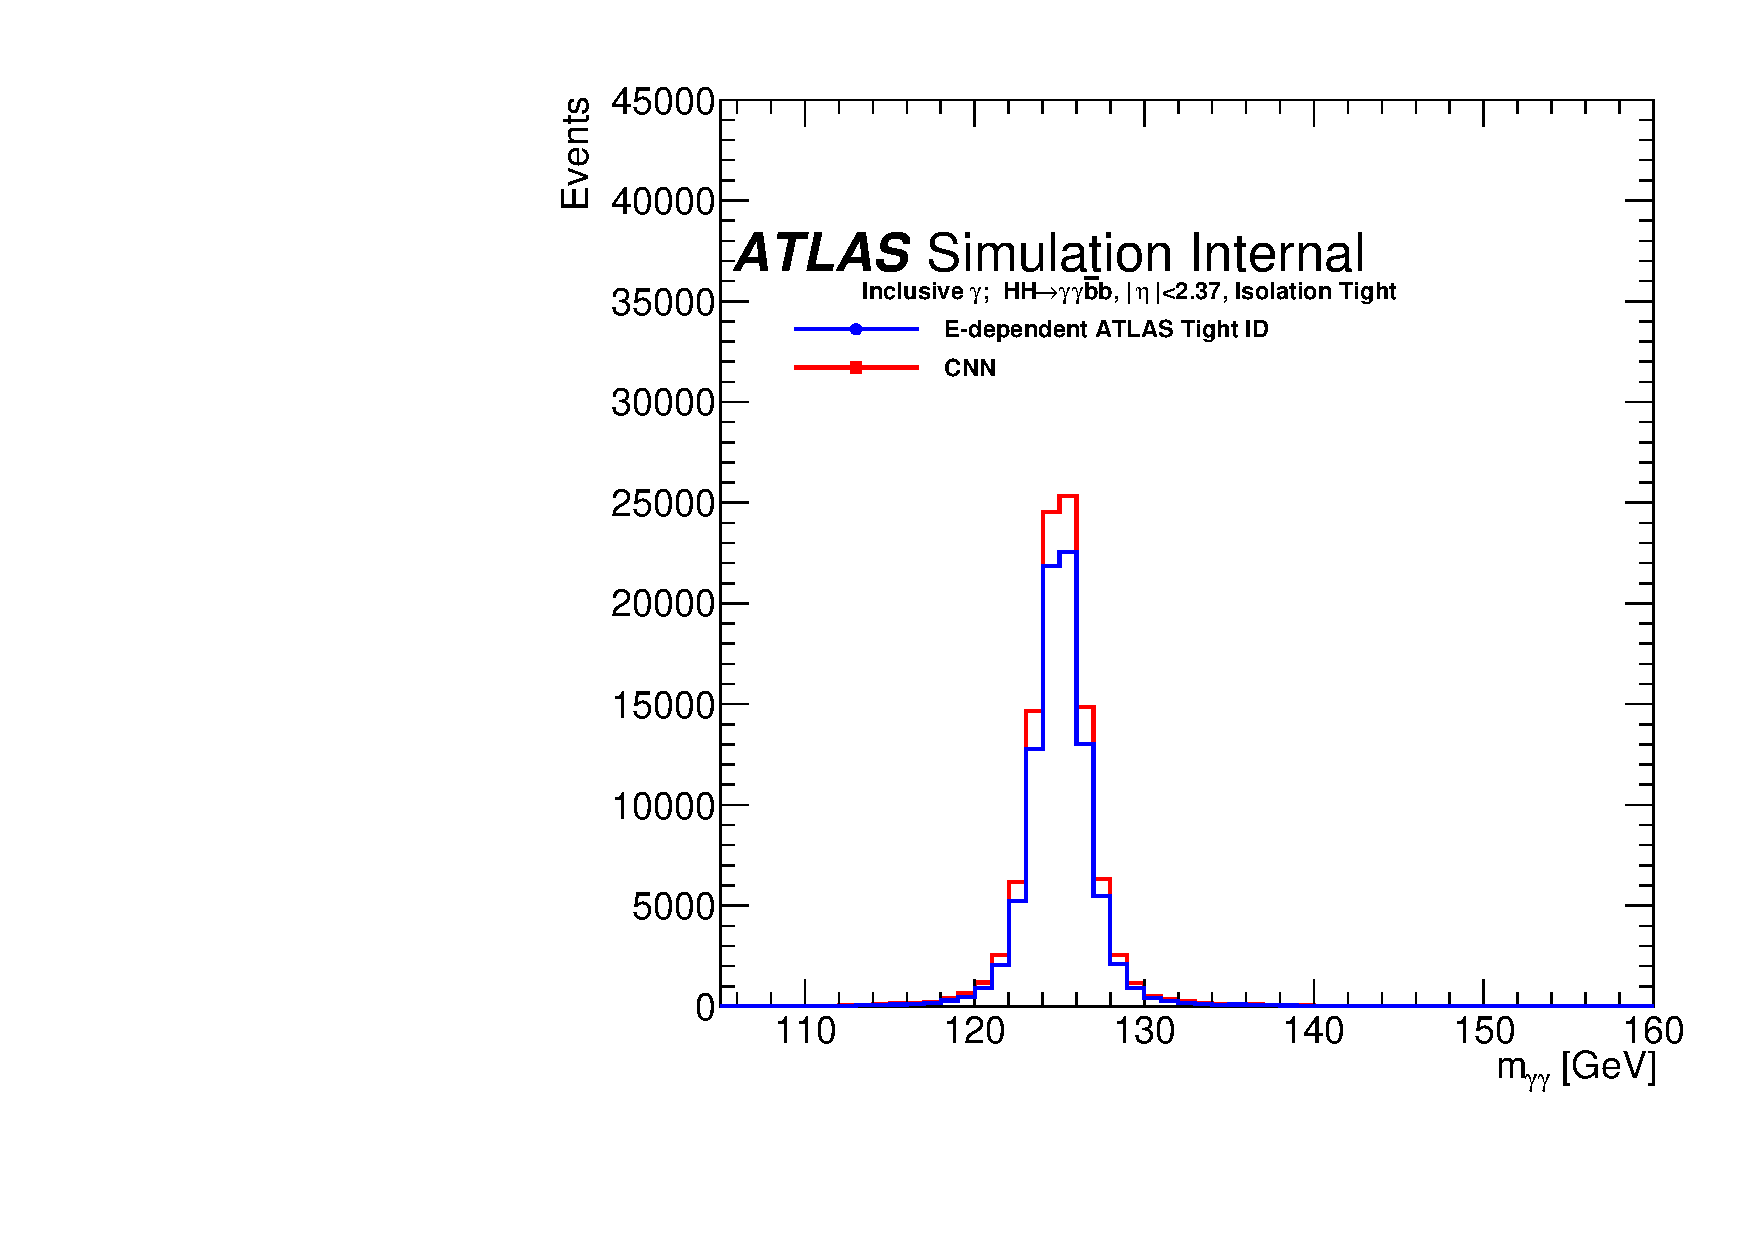
\includegraphics[width=1\textwidth]{Part6/Img/Eff_Tight_All_Inclusive_Tight_M_Sig.pdf}}
    \onslide<5>\centering\fcolorbox{HHturquoise_m}{HHwhite2}{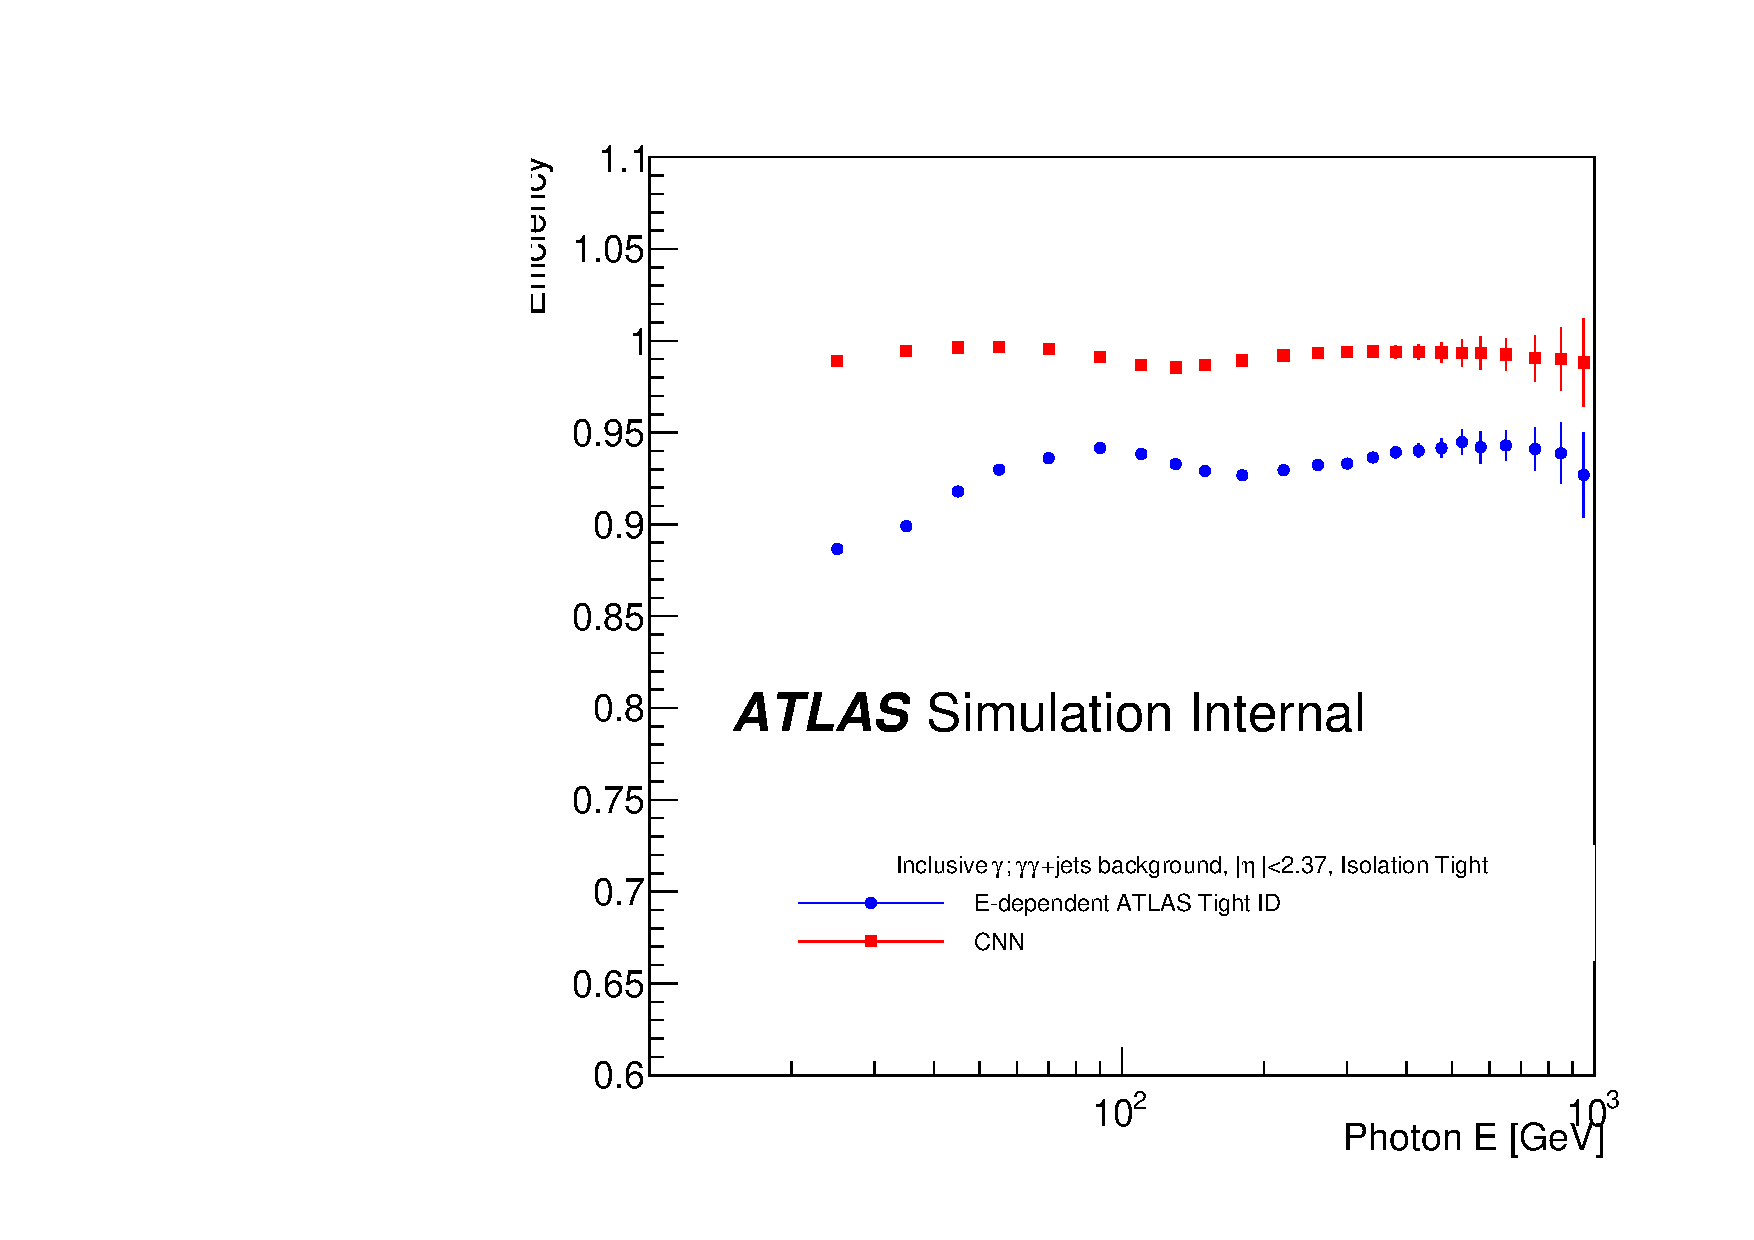
\includegraphics[width=1\textwidth]{Part6/Img/Eff_Tight_All_Inclusive_Tight_E_Bkg.pdf}}
    \onslide<6>\centering\fcolorbox{HHturquoise_m}{HHwhite2}{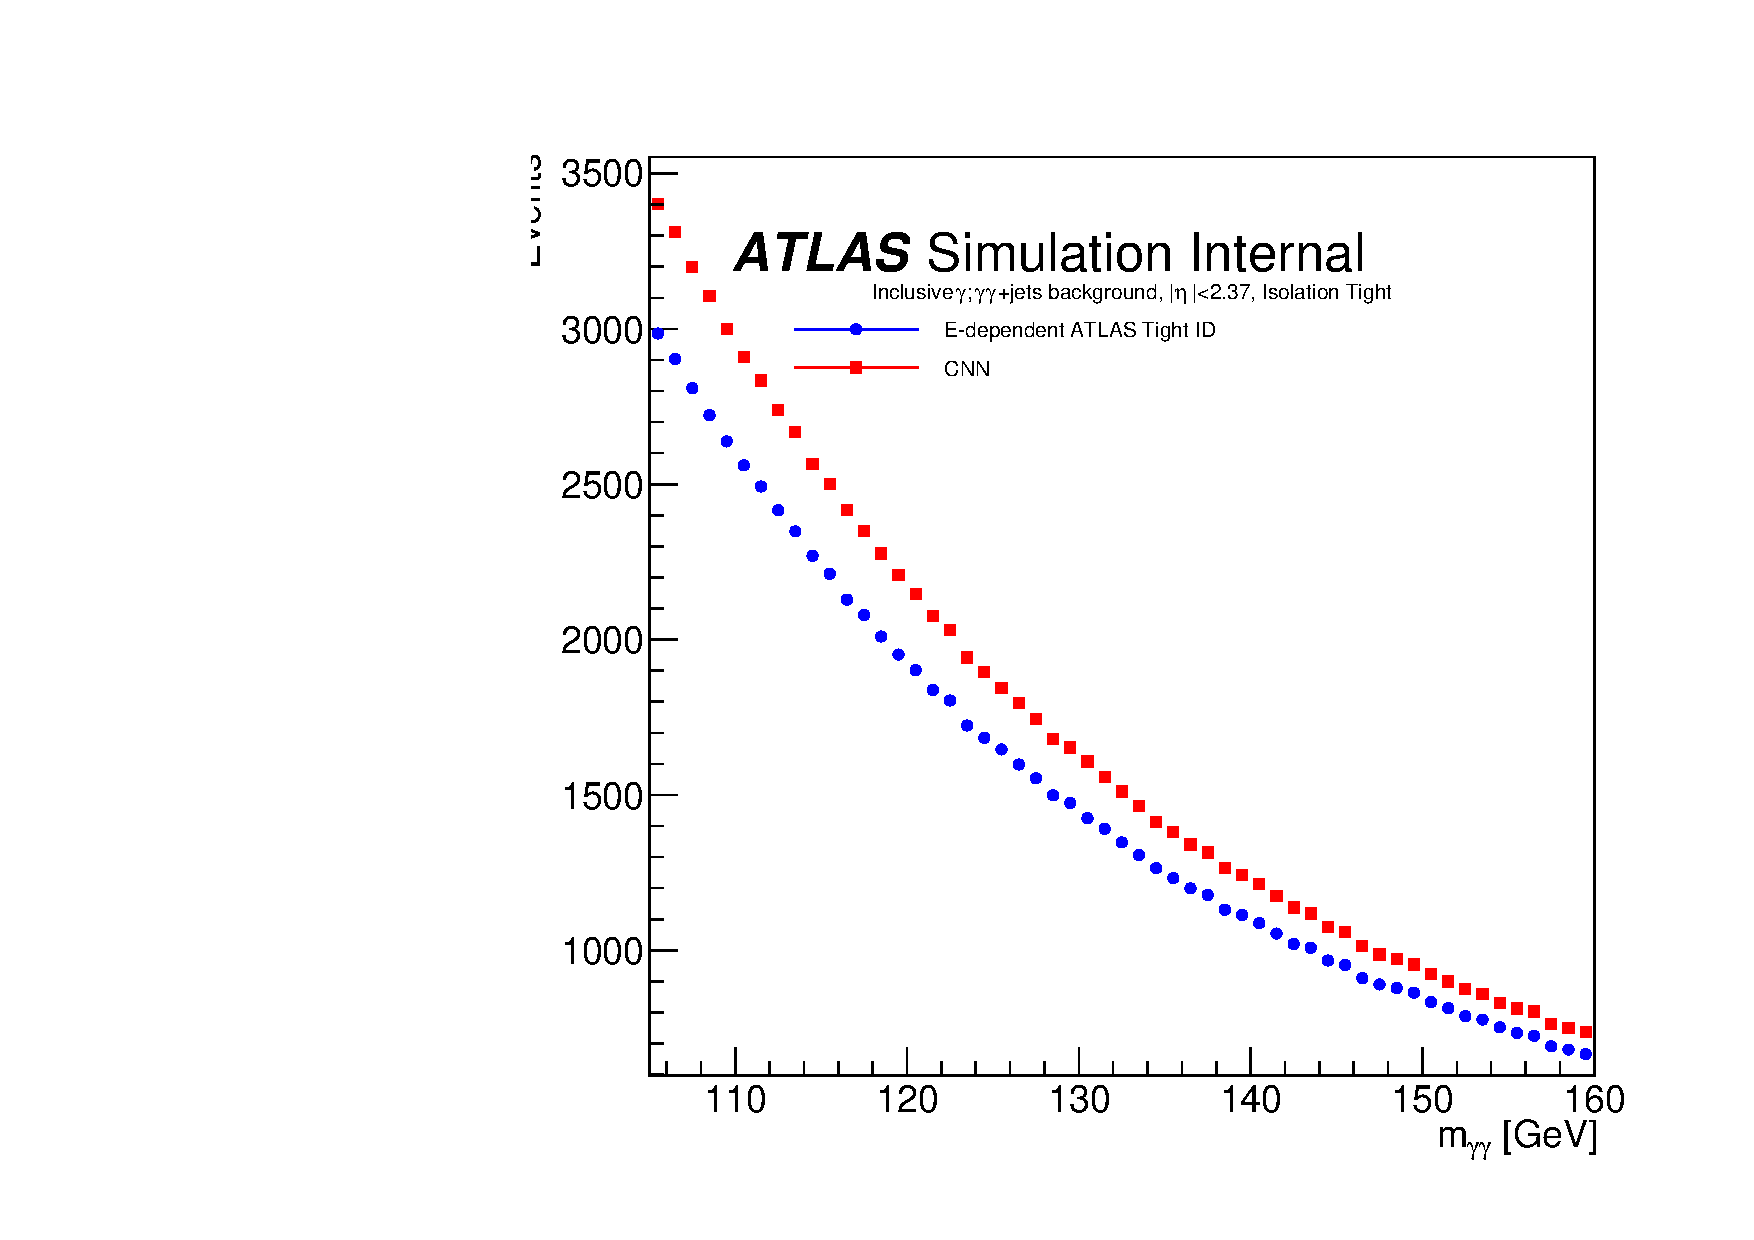
\includegraphics[width=1\textwidth]{Part6/Img/Eff_Tight_All_Inclusive_Tight_M_Bkg.pdf}}
    \end{overprint}
\end{figure}
\end{columns}

\end{frame}

\subsection{Future improvement}
\begin{frame}{Future improvement}
    \textbf{Is really needed}
\end{frame}